\section{Theory}

	\subsection{Annihilation Radiation}
		Coincidence refers to the simultaneous detection of the gamma that was released after the decay but in the opposite direction. The probability distribution for the decay of $Na^{22}$ nuclei is $90\%$ positron emission and $10\%$ electron capture, as illustrated in the \hyperref[fig:1]{Fig 1}.
		\begin{figure}[h]
			\centering
			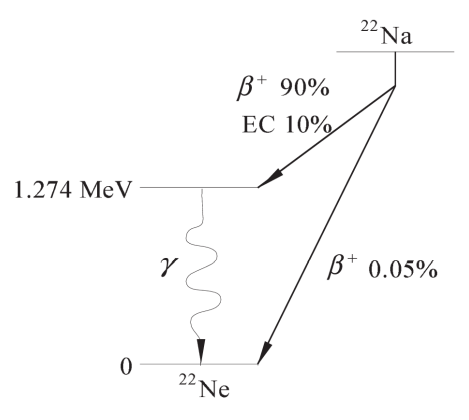
\includegraphics[width=0.8\columnwidth]{images/theory1.png}
			\caption{\textbf{Decay of $Na^{22}$}}
			\label{fig:1}
		\end{figure}

		The ensuing $Na^{22}$ nucleus deexcites to its ground state with the emission of a $1.274 MeV$ gamma ray with a mean lifetime of 3 picoseconds. Sodium Iodide scintillators and a photomultimeter are used to detect these gamma emissions. Using computer software, the output signal is amplified and presented as a histogram. The positrons are released with a variety of kinetic energy up to approximately a half mega electron volts, which they lose in the surrounding material at a rate of roughly one nanosecond, reducing to atomic energies in electron volts. To create positronium, a hydrogen-like "atom" with a lifespan of $10^-{10}$s, they now catch an electron. This decay is caused by the annihilation of the positron and electron into two gammas.

		Since the positron is at rest in its frame, the conservation of energy and momentum requires that the gamma be emitted in the opposite direction ($180^\circ$) with equal kinetic energies, allowing for simultaneous detection in the detectors placed on both sides of the sample. Apiece gamma will have an energy $E_{\gamma} = 0.511\; MeV$ since the beginning energy of the positronium (ignoring the binding energy of a few eV) is only the rest mass energy of an electron and positron ($0.511MeV$ each). However, the situation would be different in the laboratory frame, where the positronium will be moving with a range of kinetic energies up to a few eV. Then, depending on the direction of the initial positronium momentum relative to the gamma emission direction, the transformation to the lab frame gives gamma energies that might differ from $0.511\;MeV$ and/or produce gammas that are not emitted exactly $180^\circ$ apart.

	\subsection{Experimental Setup}
		The experimental setup is similar to that of Gamma ray spectroscopy and is shown in \hyperref[fig:2]{Fig 2}. 
		\begin{figure}[h]
			\centering
			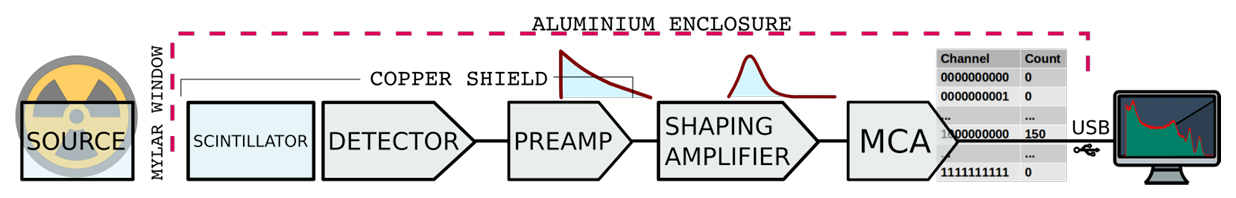
\includegraphics[width=0.9\columnwidth]{images/theory2.png}
			\caption{\textbf{\small{Flow diagram for the entire process}}}
			\label{fig:2}
		\end{figure}

		It is made up of a detector with an 8mm-diameter entrance window that is coated in aluminium to block out visible light. Inside, a semiconductor PN junction coupled in reverse bias mode is mated to a scintillator that measures 10mm by 10mm by 8mm. It is a Sodium Iodide scintillator with Thorium doping that emits photons with the same energy as the gamma ray's descent. The scintillation photons are transformed into an equivalent amount of electron-hole pairs in the depletion area of the PN junctions. An event in the photopeak area is caused by the little amount of charge produced when one gamma ray deposits its whole energy in the scintillator and is subsequently transformed into a charge pulse by the PN junction. A charge sensitive preamplifier receives the charge pulse and converts it into a matching output voltage to produce a spectrum. The Shaping Amplifier then generates a pulse with a Guassian form. Depending on the amount of energy deposited, the amplitude ranges from 0 to 3.3 volts. The same buffered signal enters the built-in Multi-Channel Analyzer (MCA), whose hardware is capable of a number of tasks including pulse detection, post-processing, and sorting signals based on peak height into predefined bins with a 10bit resolution. The input voltage range for the MCA is 0 to 3.3V. The programme CNSPEC includes a wide range of tools for data analysis and can plot the obtained data in real-time.

	\subsection{Coincidence Rate}
		The nuclear decay rate (number of nuclear decays per second) is $\tau_n\; =\; \alpha \dot3.7 \cross 10^{10} decays/sec/curie$, where $\alpha$ is the source activity in curies. For the $90\%$ probability of gamma emission, the rate of emission of $0.511\; MeV$ gammas is $1.8\;\tau_n$. These gammas are emitted uniformly (in oppositely directed pairs) from	the source. Thus at a distance R from the source they are spread out over an area $4\pi R^2$ and the flux $\phi$ (number per unit area per second) will be:
		
		$$\phi =\; 1.8\tau_n4\pi R^2$$

		The apertures, the scintillators and their relationship to the source and each other are an important factor in determining the rates at which gammas are detected. The fraction of $0.511\; MeV$ gammas which get through the lead shielding will also need to be specified. It is expected to be on the order of $20\%$ and will be expressed by the symbol $\kappa$.

		With these considerations, the rate $Q$ of $0.511\; MeV$ gammas striking the face of the scintillator can be calculated. 
		
		$$Q\;=\; \phi[A_a + \kappa(A_s - A_a)]$$

		where the area of the aperture is $A_a = \pi r_a^2$, and the area of the scintillator is $A_s = \pi r^2_s$, where $r_i$ are the respective radii.